
\documentclass{article}


\usepackage{amssymb,amsmath,mathtools,xcolor,graphicx,xspace,colortbl,ragged2e,rotating} 
\usepackage{amsfonts}  
\usepackage{boxedminipage} 
\usepackage{graphics}  
\usepackage{ragged2e}
\usepackage{wrapfig}  
\usepackage{xcolor}  
\graphicspath{{images/}}
\DeclareGraphicsExtensions{.pdf,.eps,.ps,.png,.jpg,.jpeg}
\begin{document}
\title{\textbf{AI1110 Assignment 1} }
\author{\textbf{Dondapati Chandrahas Reddy}\\\textbf{AI21BTECH11010}}
\maketitle
\begin{center}
{\Large ICSE Grade 10 2019 paper
}\end{center}\par
{\Large 

\section{Question 3 (a) }
}{\Large \underline{Question}:}


\begin{center}
\setlength \fboxrule {0in}
\setlength \fboxsep {0.1in}
\fcolorbox[HTML]{FFFFFF}{FFFFFF}{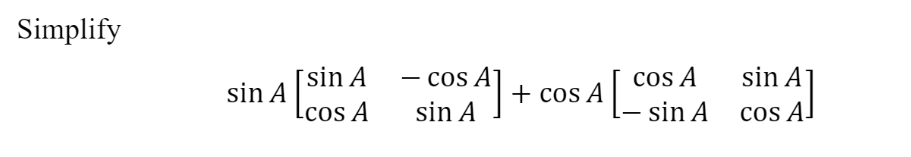
\includegraphics [ width=5.8125in, height=1in,]{img1} }
\end{center}\par
{\Large \underline{Solution:}\newline\newline}
Performing scalar multiplication we get 


\begin{center}
$\left [\begin{array}{cc}\sin ^{2} A &  -\sin  A \cos  A \\
\sin  A \cos  A & \sin ^{2} A\end{array}\right ] +\left [\begin{array}{cc}\cos ^{2} A & \cos  A \sin  A \\
 -\cos  A \sin  A & \cos ^{2} A\end{array}\right ]$\newline
\end{center}\par
Adding the matrices 


\begin{center}
$\left [\begin{array}{cc}\sin ^{2} A +\cos ^{2} A &  -\sin  A \cos  A +\cos  A \sin  A \\
\sin  A \cos  A -\cos  A \sin  A & \sin ^{2} A +\cos ^{2} A\end{array}\right ]$\linebreak\relax
\end{center}\par
Simplifying the expressions we get



\begin{center}
$\left [\begin{array}{cc}1 & 0 \\
0 & 1\end{array}\right ]$
\end{center}\par
\end{document}